% $Id$
%==============================================================================
\section{A Local Component's Structure}
\label{ComponentStructure}
%==============================================================================

The implementation of server--side components is made up of different parts,
as shown in Fig.~\ref{ContainerComponentlogicBusinesslogic}, that are either
manually written, generated by tools or existing libraries.

\begin{figure}[htbp]
    \begin{center}
    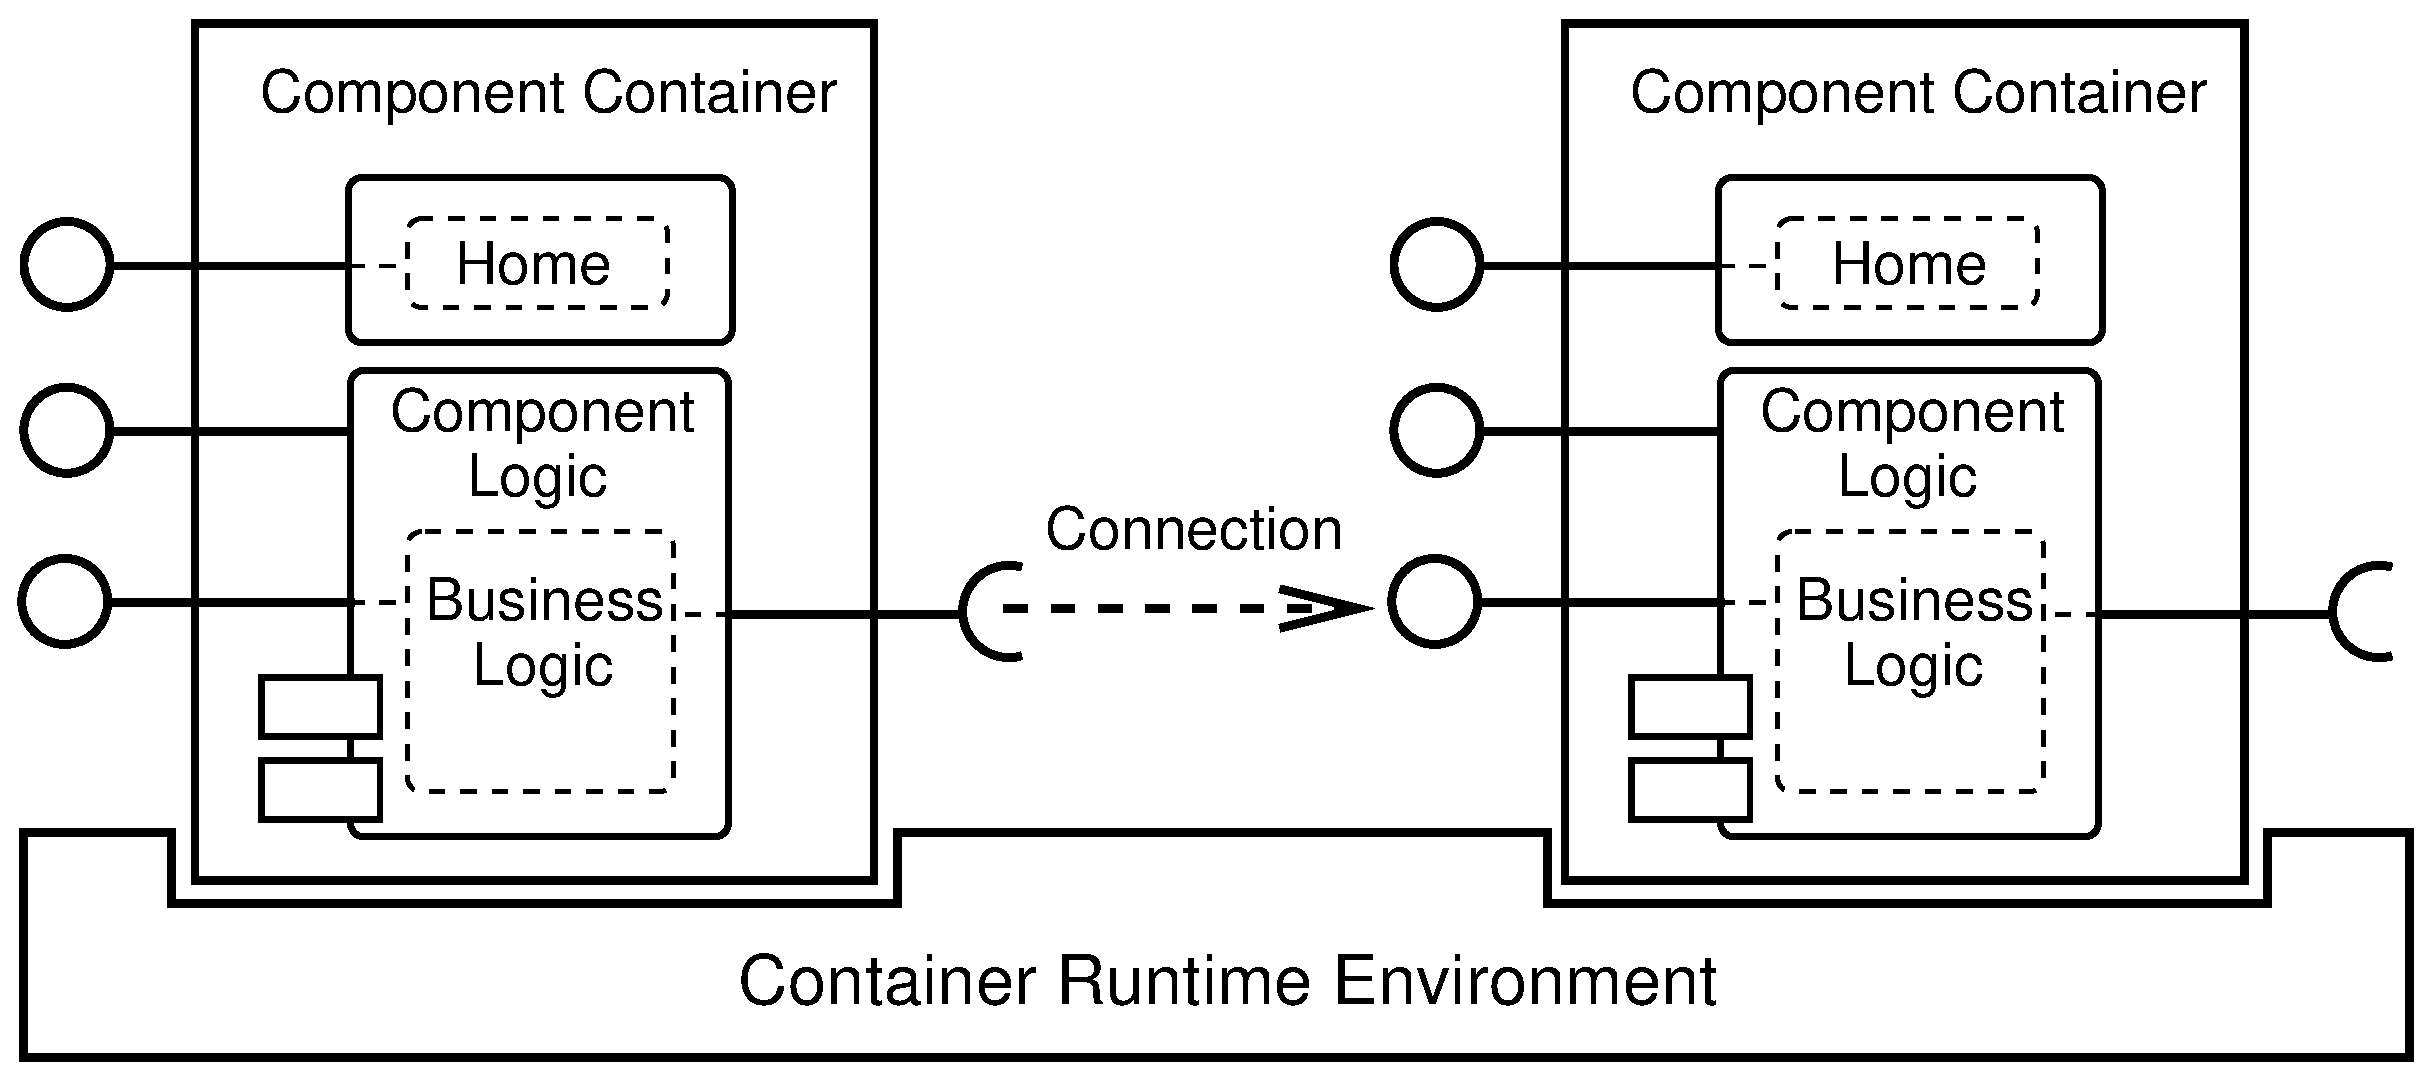
\includegraphics [width=10cm,angle=0] 
		     {figures/ContainerComponentlogicBusinesslogic.eps}
    \caption{A component implementation covers business logic, component
    logic, component container and container runtime environment.}
    \label{ContainerComponentlogicBusinesslogic}            
    \end{center}
\end{figure}

\begin{description}
\item [Business logic:]
  a component's business logic is written by the component developer to 
  implement   a domain specific functionality.
  Basically, business logic should not deal with technical aspects like contract
  verification or middleware API.
  
\item [Component logic:]
  business logic is embedded in a layer of generated code called component 
  logic. The interaction between business logic and component logic is well 
  defined in terms of interfaces (context interface, callback interface).
  Component logic handles technical aspects as well as a component's life-cycle.
  Additionally, component logic is glue code that fits a component into a 
  generic component container.
  
\item [Component container:]
  a component type is hosted by a component container that manages instances of
  that component type.
  While component logic is generated for each particular component type, the 
  component container is a generic part of the component platform.
  
\item [Container runtime environment:]
  a component platform also supports a set of libraries and services that can 
  be used by component containers.
  Any middleware used here is also part of this runtime environment.
\end{description}


\noindent
From this implementation schema, two different component views can be deduced:
\begin{description}
\item [External view:]
  a component provides its ports defined by interfaces. All 
  client calls to these ports are routed through the component container and 
  the generated component logic before business logic functionality is
  executed.
  
\item [Internal view:]
  a component's business logic can call methods on a context 
  object, which is part of generated component logic, and has to implement 
  a callback interface that allows the component container to handle the 
  component's life--cycle.
\end{description}


\noindent
Conforming with the concept of component model and 
middleware separation, we have implemented a local version of LwCCM components.
These local components host business logic and are completely independent 
from a particular middleware technology.

\begin{figure}[htbp]
    \begin{center}
    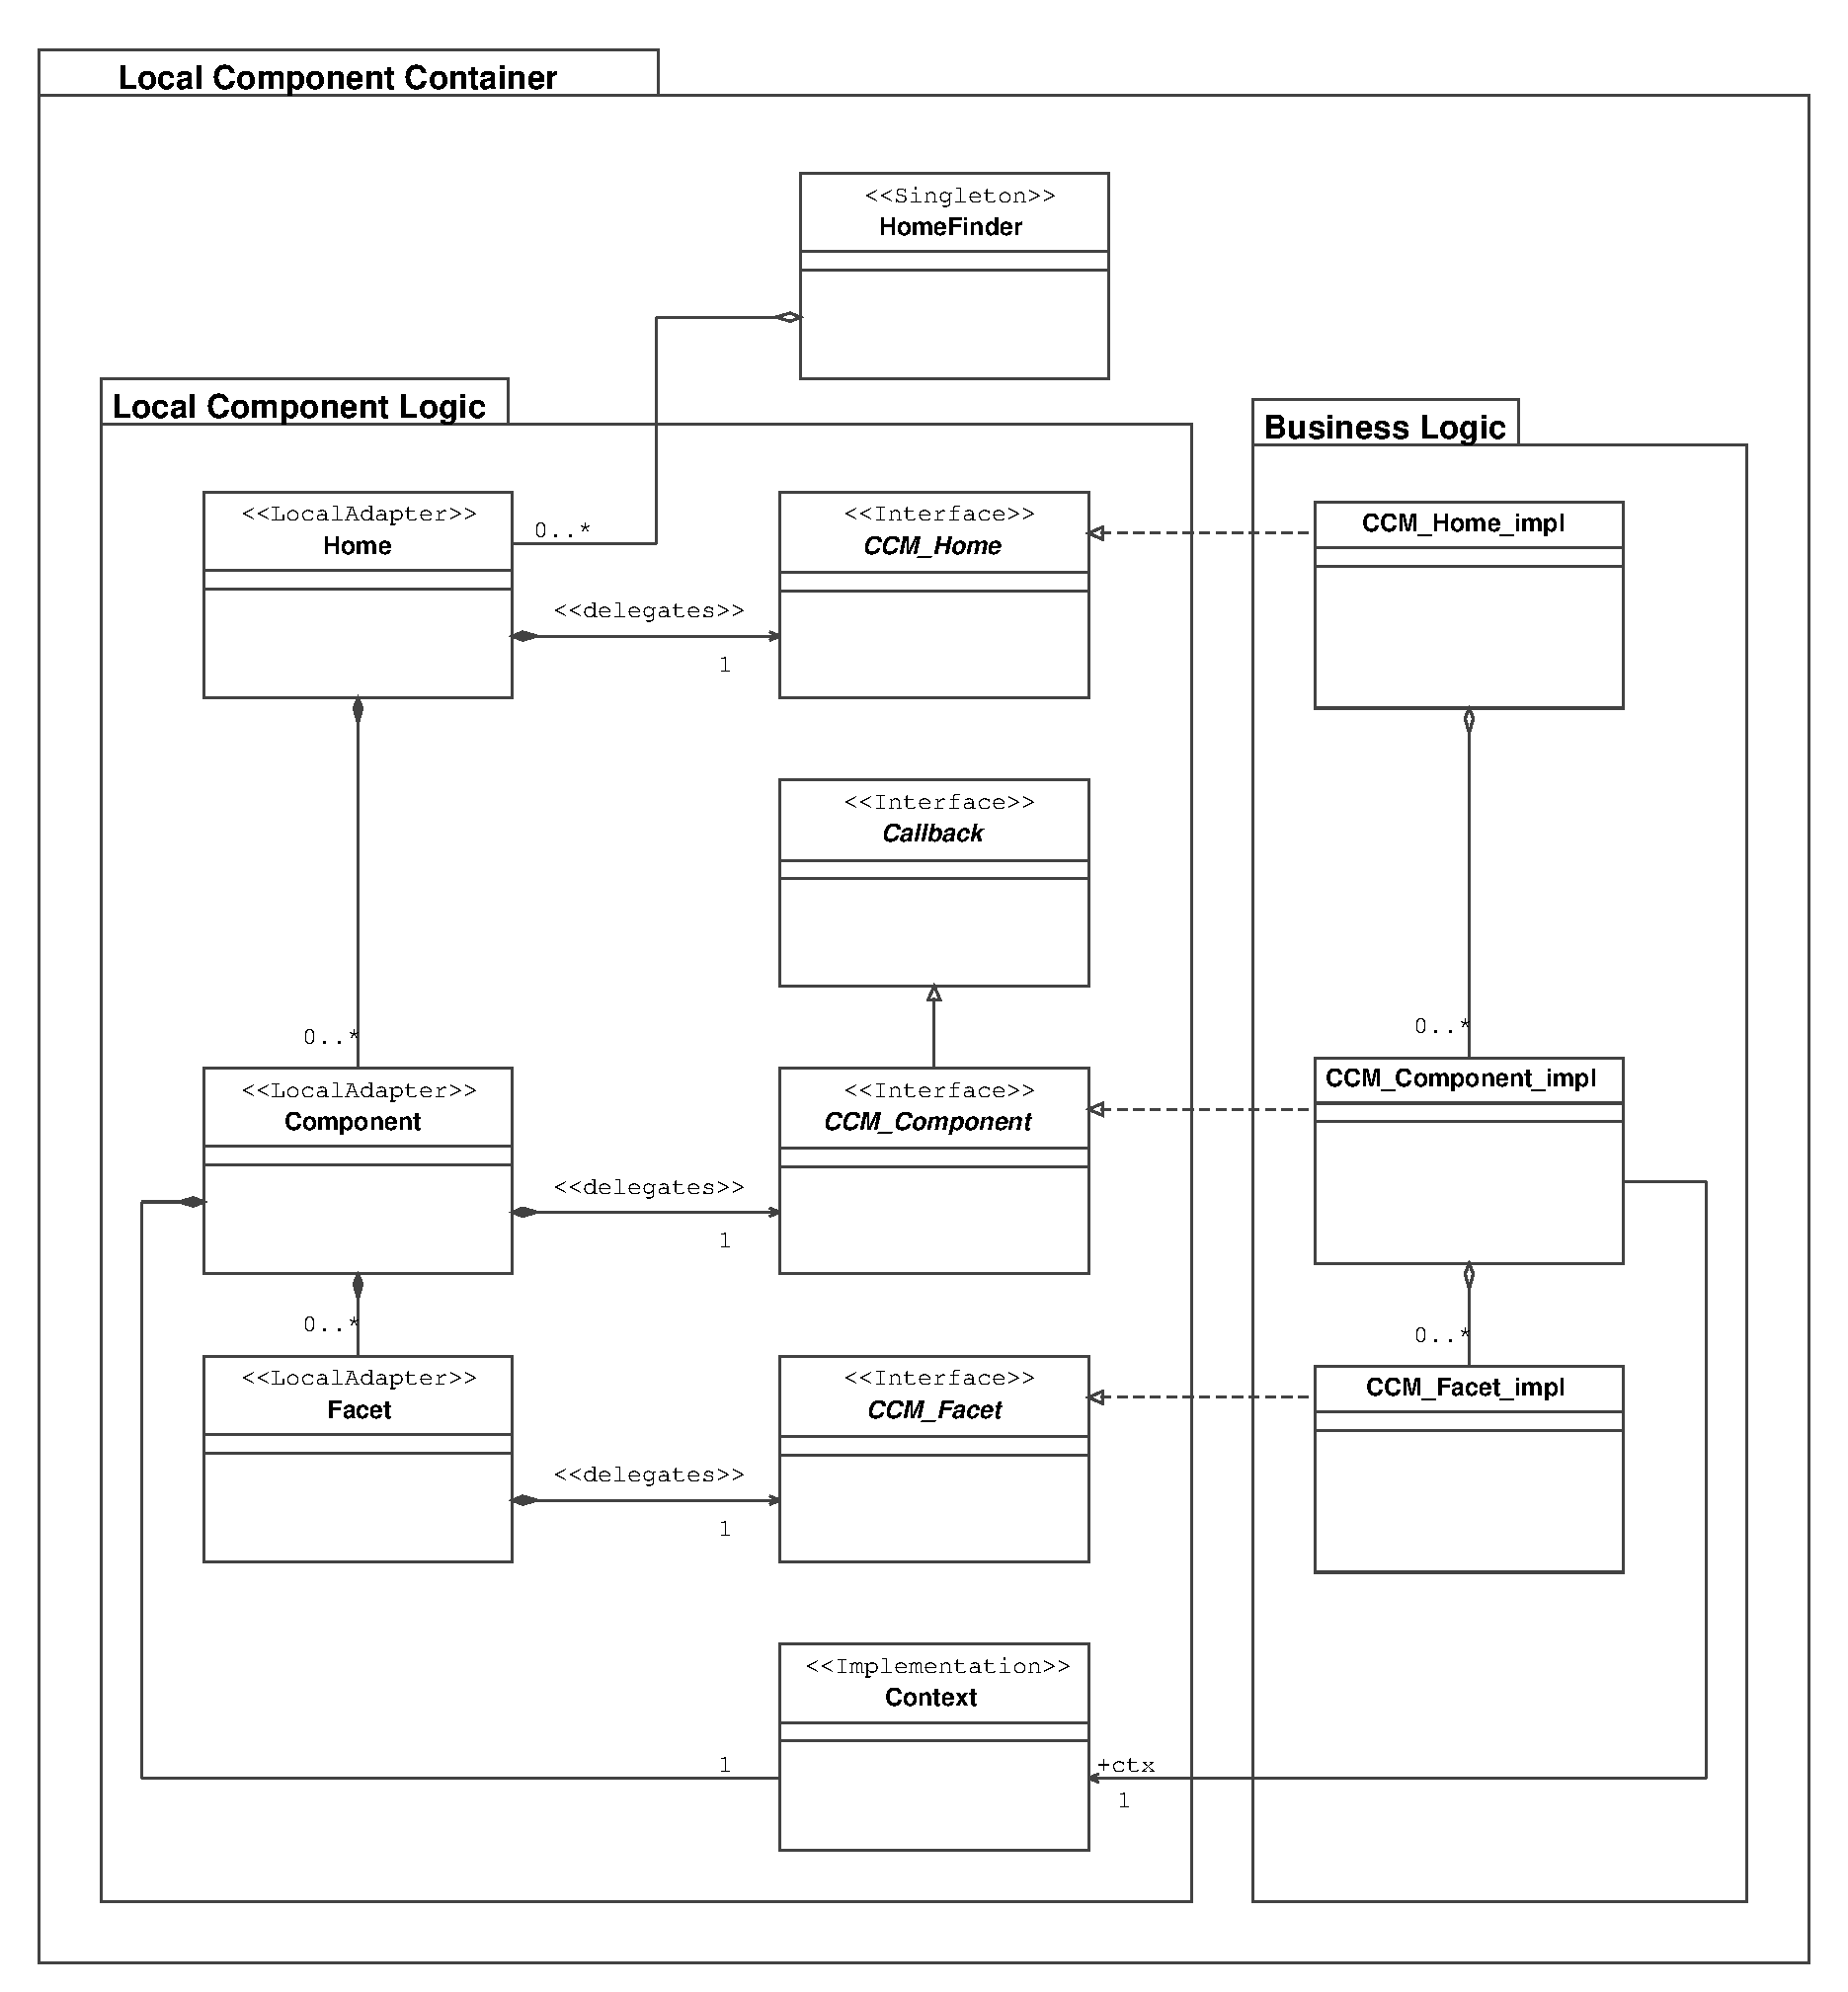
\includegraphics [width=15cm,angle=0] {uml/StructureOfLocalComponents.eps}
    \caption{This simplified structure of a local component implementation
    shows the relationship between business logic, local component logic and
    a local component container.}
    \label{StructureOfLocalComponents}            
    \end{center}
\end{figure}

\noindent
Implementations without middleware are much leaner and allow
finer grained components which are simpler to reuse.
Especially in languages that do not provide a native component model
(like C++), a local version of LwCCM can be useful.  

\newpage
\noindent
Based on this simplified class diagram, we can analyze the following
interactions between business logic and component logic:

\begin{description}
\item [Calling component methods:]
usually, a component client calls methods on a component's interface.
These interfaces can be either a component home, a component equivalent 
interface or a facet.
Invocations on all these interfaces follow the same structural pattern,
as shown in Fig.~\ref{LocalComponentImplementationStructure}.
A component's client calls methods on generated adapter classes 
that implements a component's interfaces. 
These adapters delegate calls 
to generated interfaces which are implemented by business logic classes.
\begin{figure}[htbp]
    \begin{center}
    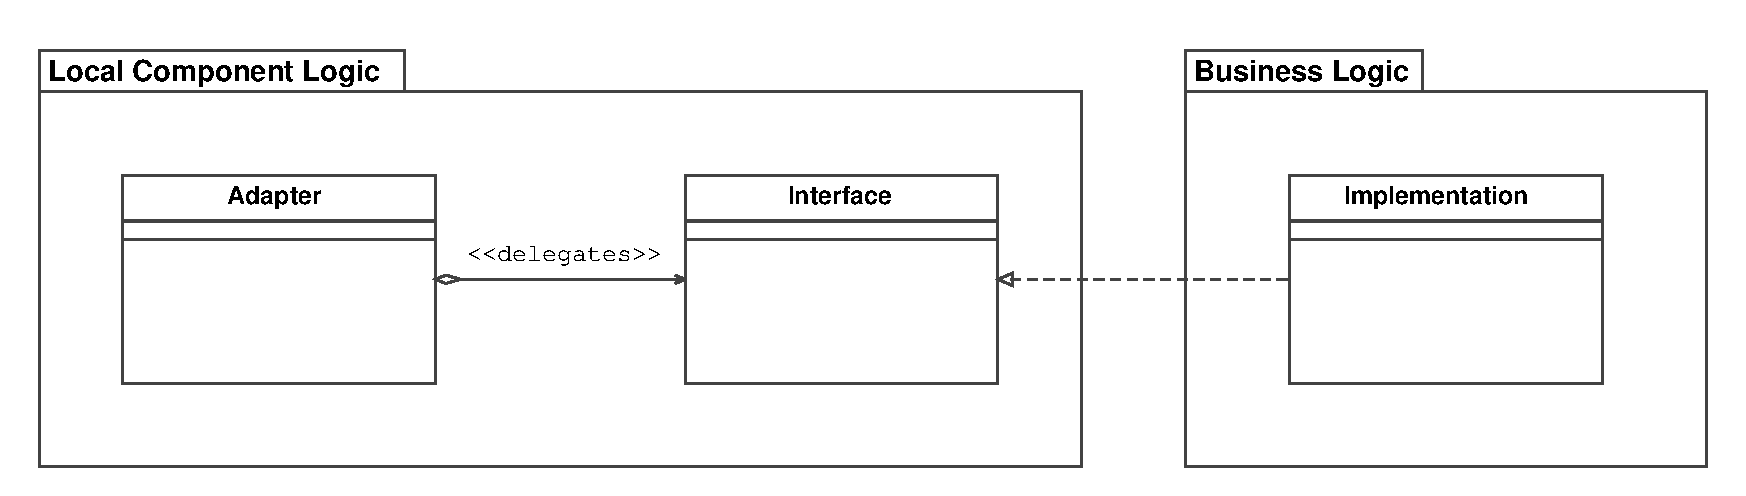
\includegraphics [width=13cm,angle=0] 
		     {uml/LocalComponentImplementationStructure.eps}
    \caption{Structure of a local component.}
    \label{LocalComponentImplementationStructure}            
    \end{center}
\end{figure}

This pattern implies two benefits:
\begin{itemize}
\item The adapter layer brings in an indirection that can be used to execute
some pre- and post-invocation functionality.  

\item Business logic can implement a well defined interface which is generated 
from the component model.
\end{itemize}

\item [Invoking callback methods:]
as shown in Fig.~\ref{StructureOfLocalComponents}, a generated component 
interface inherits the {\tt Callback} interface that defines methods which 
will be used by the component logic to control the business logic life-cycle.

\item [Using context methods:]
while calls from component clients as well as calls from component logic to 
the callback interface 
are directed from outside to the business logic, there is also
a need for interaction between business logic and generated glue code.

In the other direction, from business logic to component logic, a {\tt Context}
object is used to provide access to container functionality.
Additionally, business logic gets receptacle references from this context 
object, that are used to call methods defined by these receptacle interfaces.
Remember, receptacles are connected to facets which implement these common
interfaces.
\end{description}

\noindent
An important part of a local component container is the {\tt HomeFinder} class. 
This class is implemented as a singleton
\cite{Gamma95} and manages component home instances.
When a local LwCCM component is deployed, an instance of the component's home
is created and registered by the {\tt HomeFinder} using a unique name. 
After that, the {\tt HomeFinder} can be used to retrieve home references by 
their name.
